\documentclass{article}
\usepackage{amsmath}
\usepackage[utf8]{inputenc}
\usepackage[margin=2cm]{geometry} 
\usepackage{graphicx}
\usepackage{placeins}
\usepackage[skip=10pt plus1pt, indent=40pt]{parskip}
\usepackage{float}
\usepackage{booktabs}
\usepackage{multicol}
\usepackage{gensymb}
\usepackage{amsmath}
\usepackage{hyperref}
\hypersetup{
    colorlinks=true,
    linkcolor=blue,
    filecolor=blue,
    citecolor=black,
    urlcolor=cyan
    }



\begin{document}

\title{Densità: misurazioni su solidi in ottone}
\author{Alessia Di Nino}
\date{30 Maggio 2023}
\maketitle

\section{Introduzione}
\subsection{Scopo dell'esperienza} %1 - alessia
L'obiettivo dell'esperienza è quello di misurare la densità dell'ottone tramite la misurazione di masse e volumi di oggetti a disposizione. 
\subsection{Cenni teorici} %2 - alessandra
Attraverso la misura del volume e della massa degli oggetti (di diverse forme) è possibile stimarne la densità. 

\begin{equation}
    \rho = \frac{m}{V}
\end{equation}

con $[\rho] = Kg/m^3$.

Infatti, dato che

\begin{equation}
    m = \rho V
\end{equation}

disponendo su un grafico cartesiano i valori dei volumi e delle masse degli oggetti di uno stesso materiale si dovrebbe ottenere una retta, passante per l'origine, che ha come coefficiente angolare proprio la densità del materiale considerato.\\ 
Dati gli oggetti a disposizione (cfr. par. \ref{subsec: metodi}) è importante tenere a mente le formule per la misura dei volumi dei seguenti solidi:

\begin{tabular}{lcl}
     \toprule
     Solido & Volume & Dimensioni\\
     \midrule
     Parallelepipedo & abc & a = altezza, b = lunghezza, c = profondità\\
     Cilindro & $\pi r^2h$ & r = raggio di base, h = altezza\\
     Prisma a base esagonale & $3b^2htan(\pi/3)$ & b = doppio dell'apotema, h = altezza\\
     \bottomrule
\end{tabular}


\FloatBarrier
 
\section{Metodi} 

\subsection{Apparato sperimentale} %3 - alessia
\label{subsec: metodi}
\begin{enumerate}
    \item Strumenti e materiale a disposizione:
    \begin{itemize}
        \item calibro ventesimale di risoluzione $0.05 mm$;
        \item calibro cinquantesimale di risoluzione $0.02 mm$;
        \item calibro palmer di risoluzione $0.01mm$;
        \item bilancia di risoluzione $0.001g$;
        \item solidi di ottone (nello specifico, un prisma a base esagonale, un parallelepipedo e quattro diversi cilindri);

    \end{itemize}

\begin{figure} [h]
    \centering
    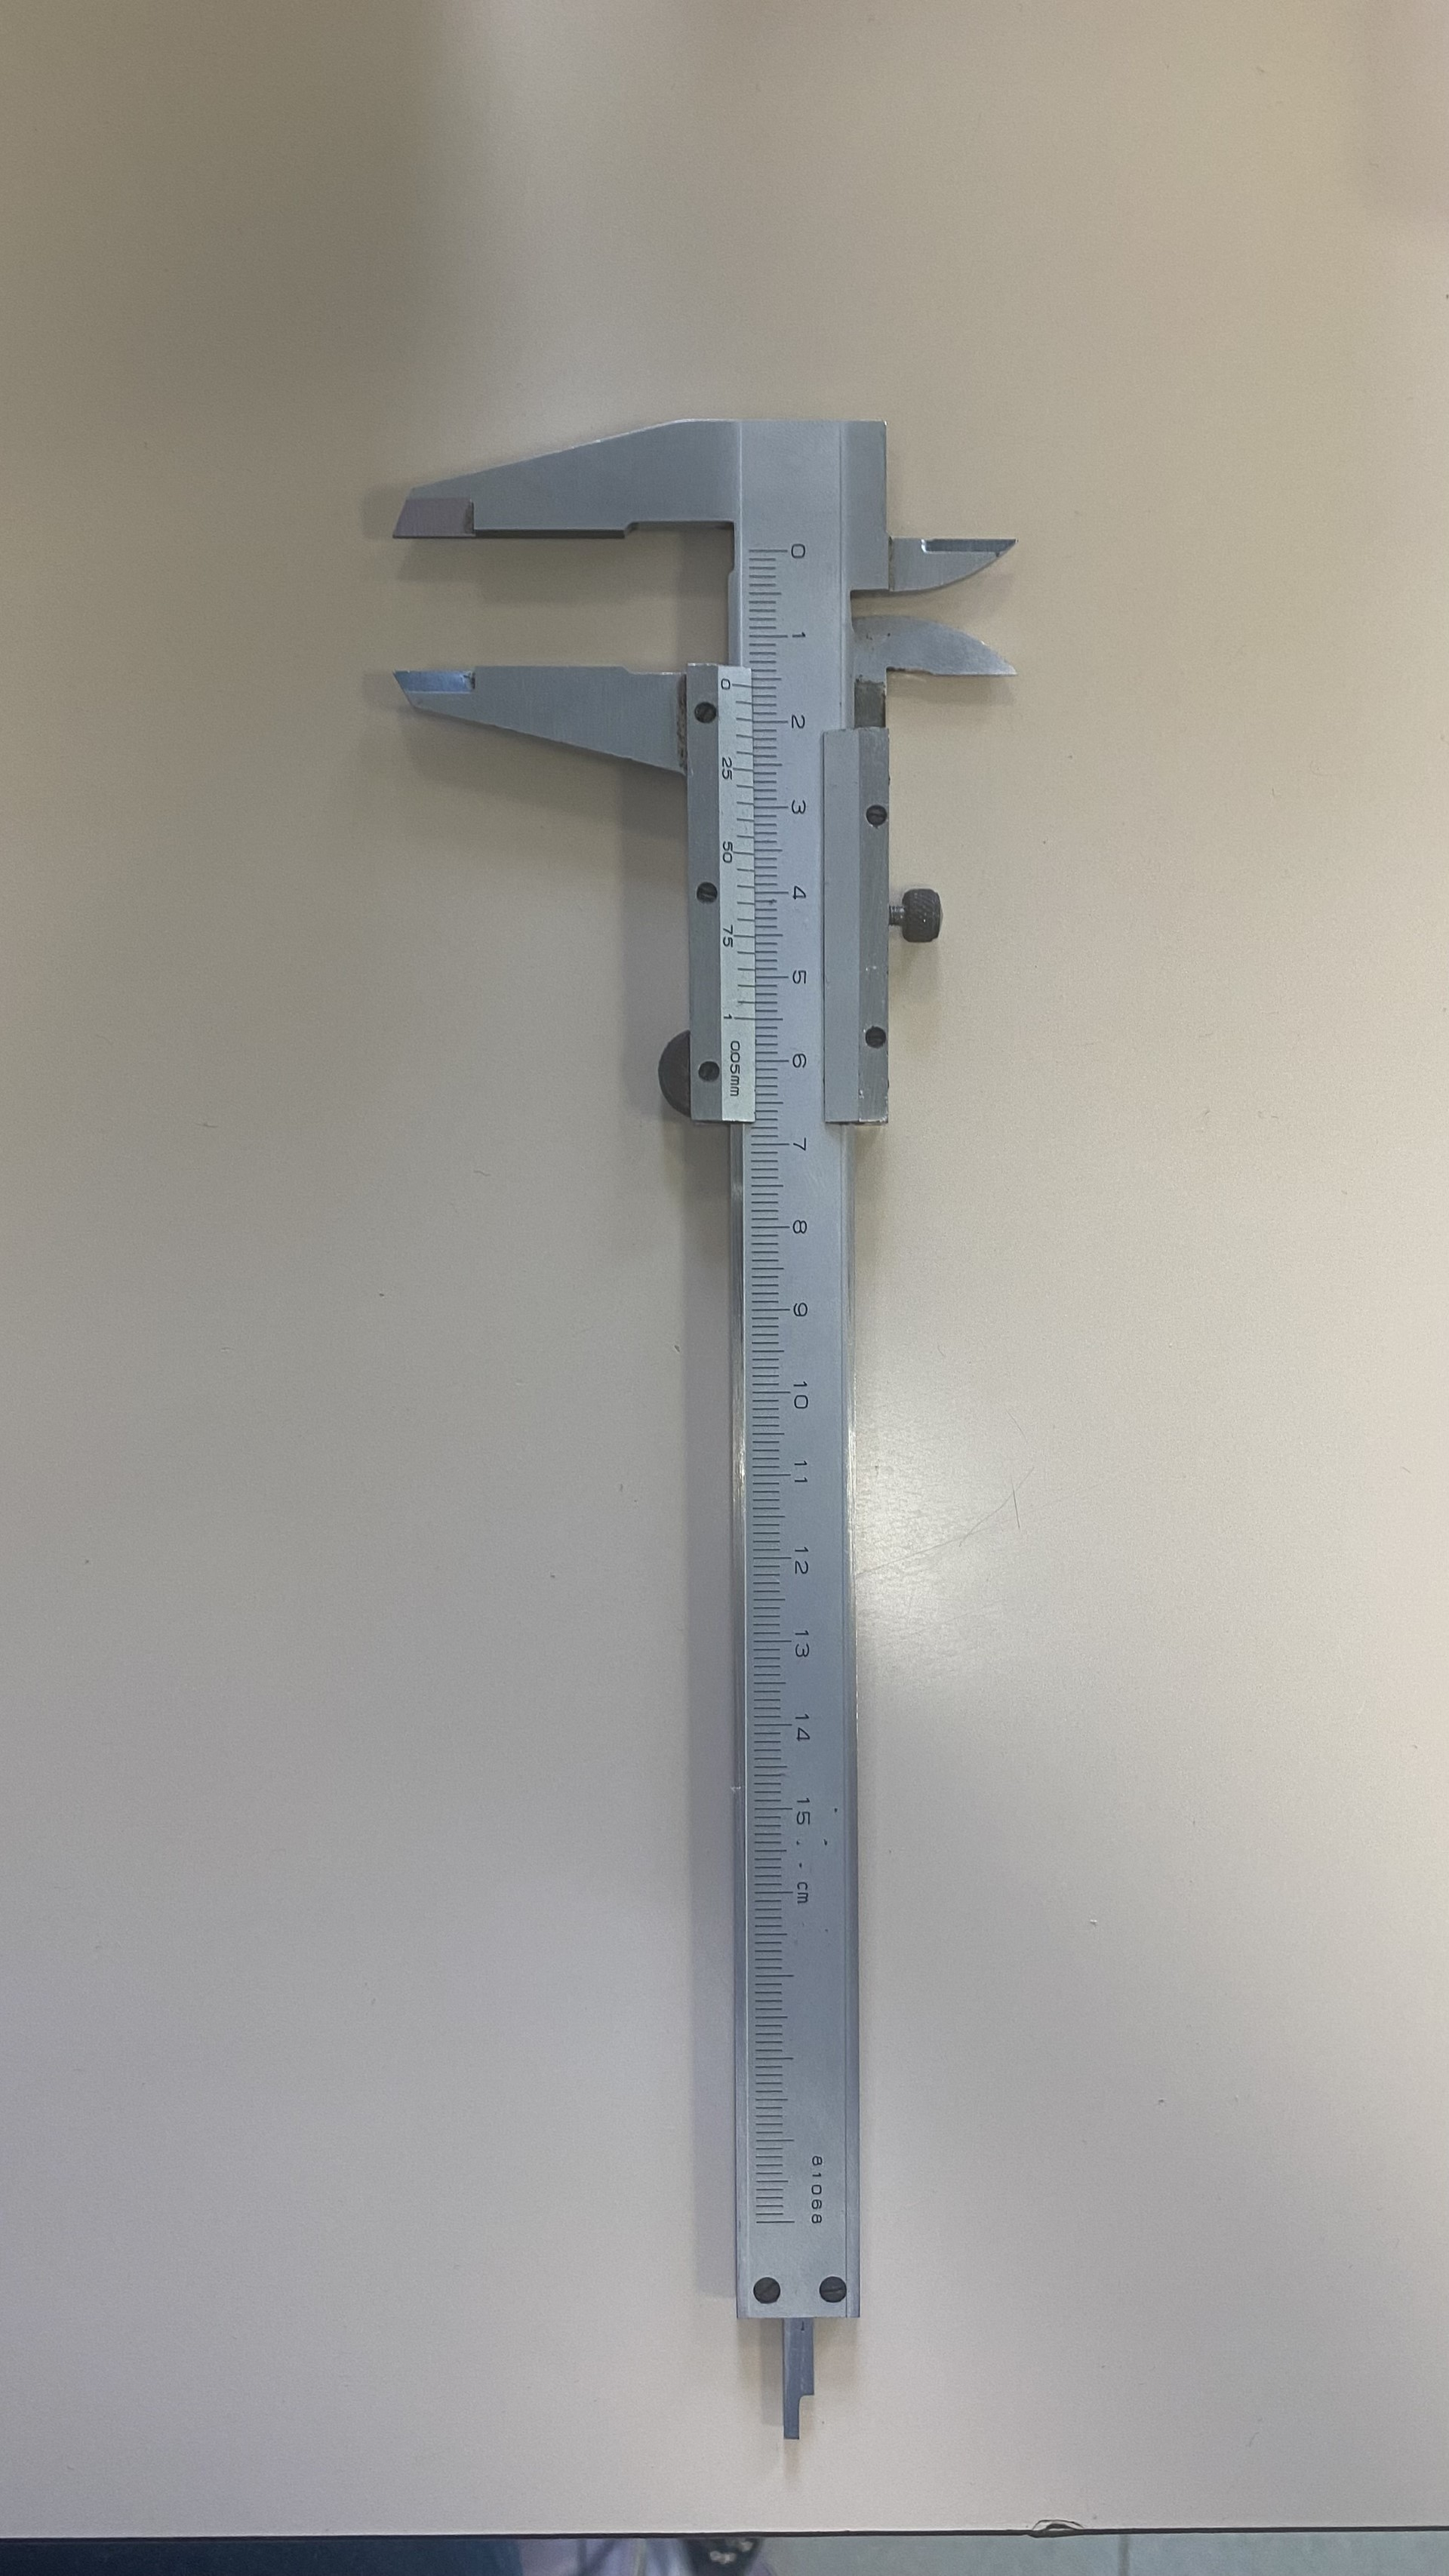
\includegraphics[width = 10cm]{calibro venti.jpg.jpg}
    \caption{Calibro ventesimale}
    \label{fig:my_label}
\end{figure}

\begin{figure}
    \centering
    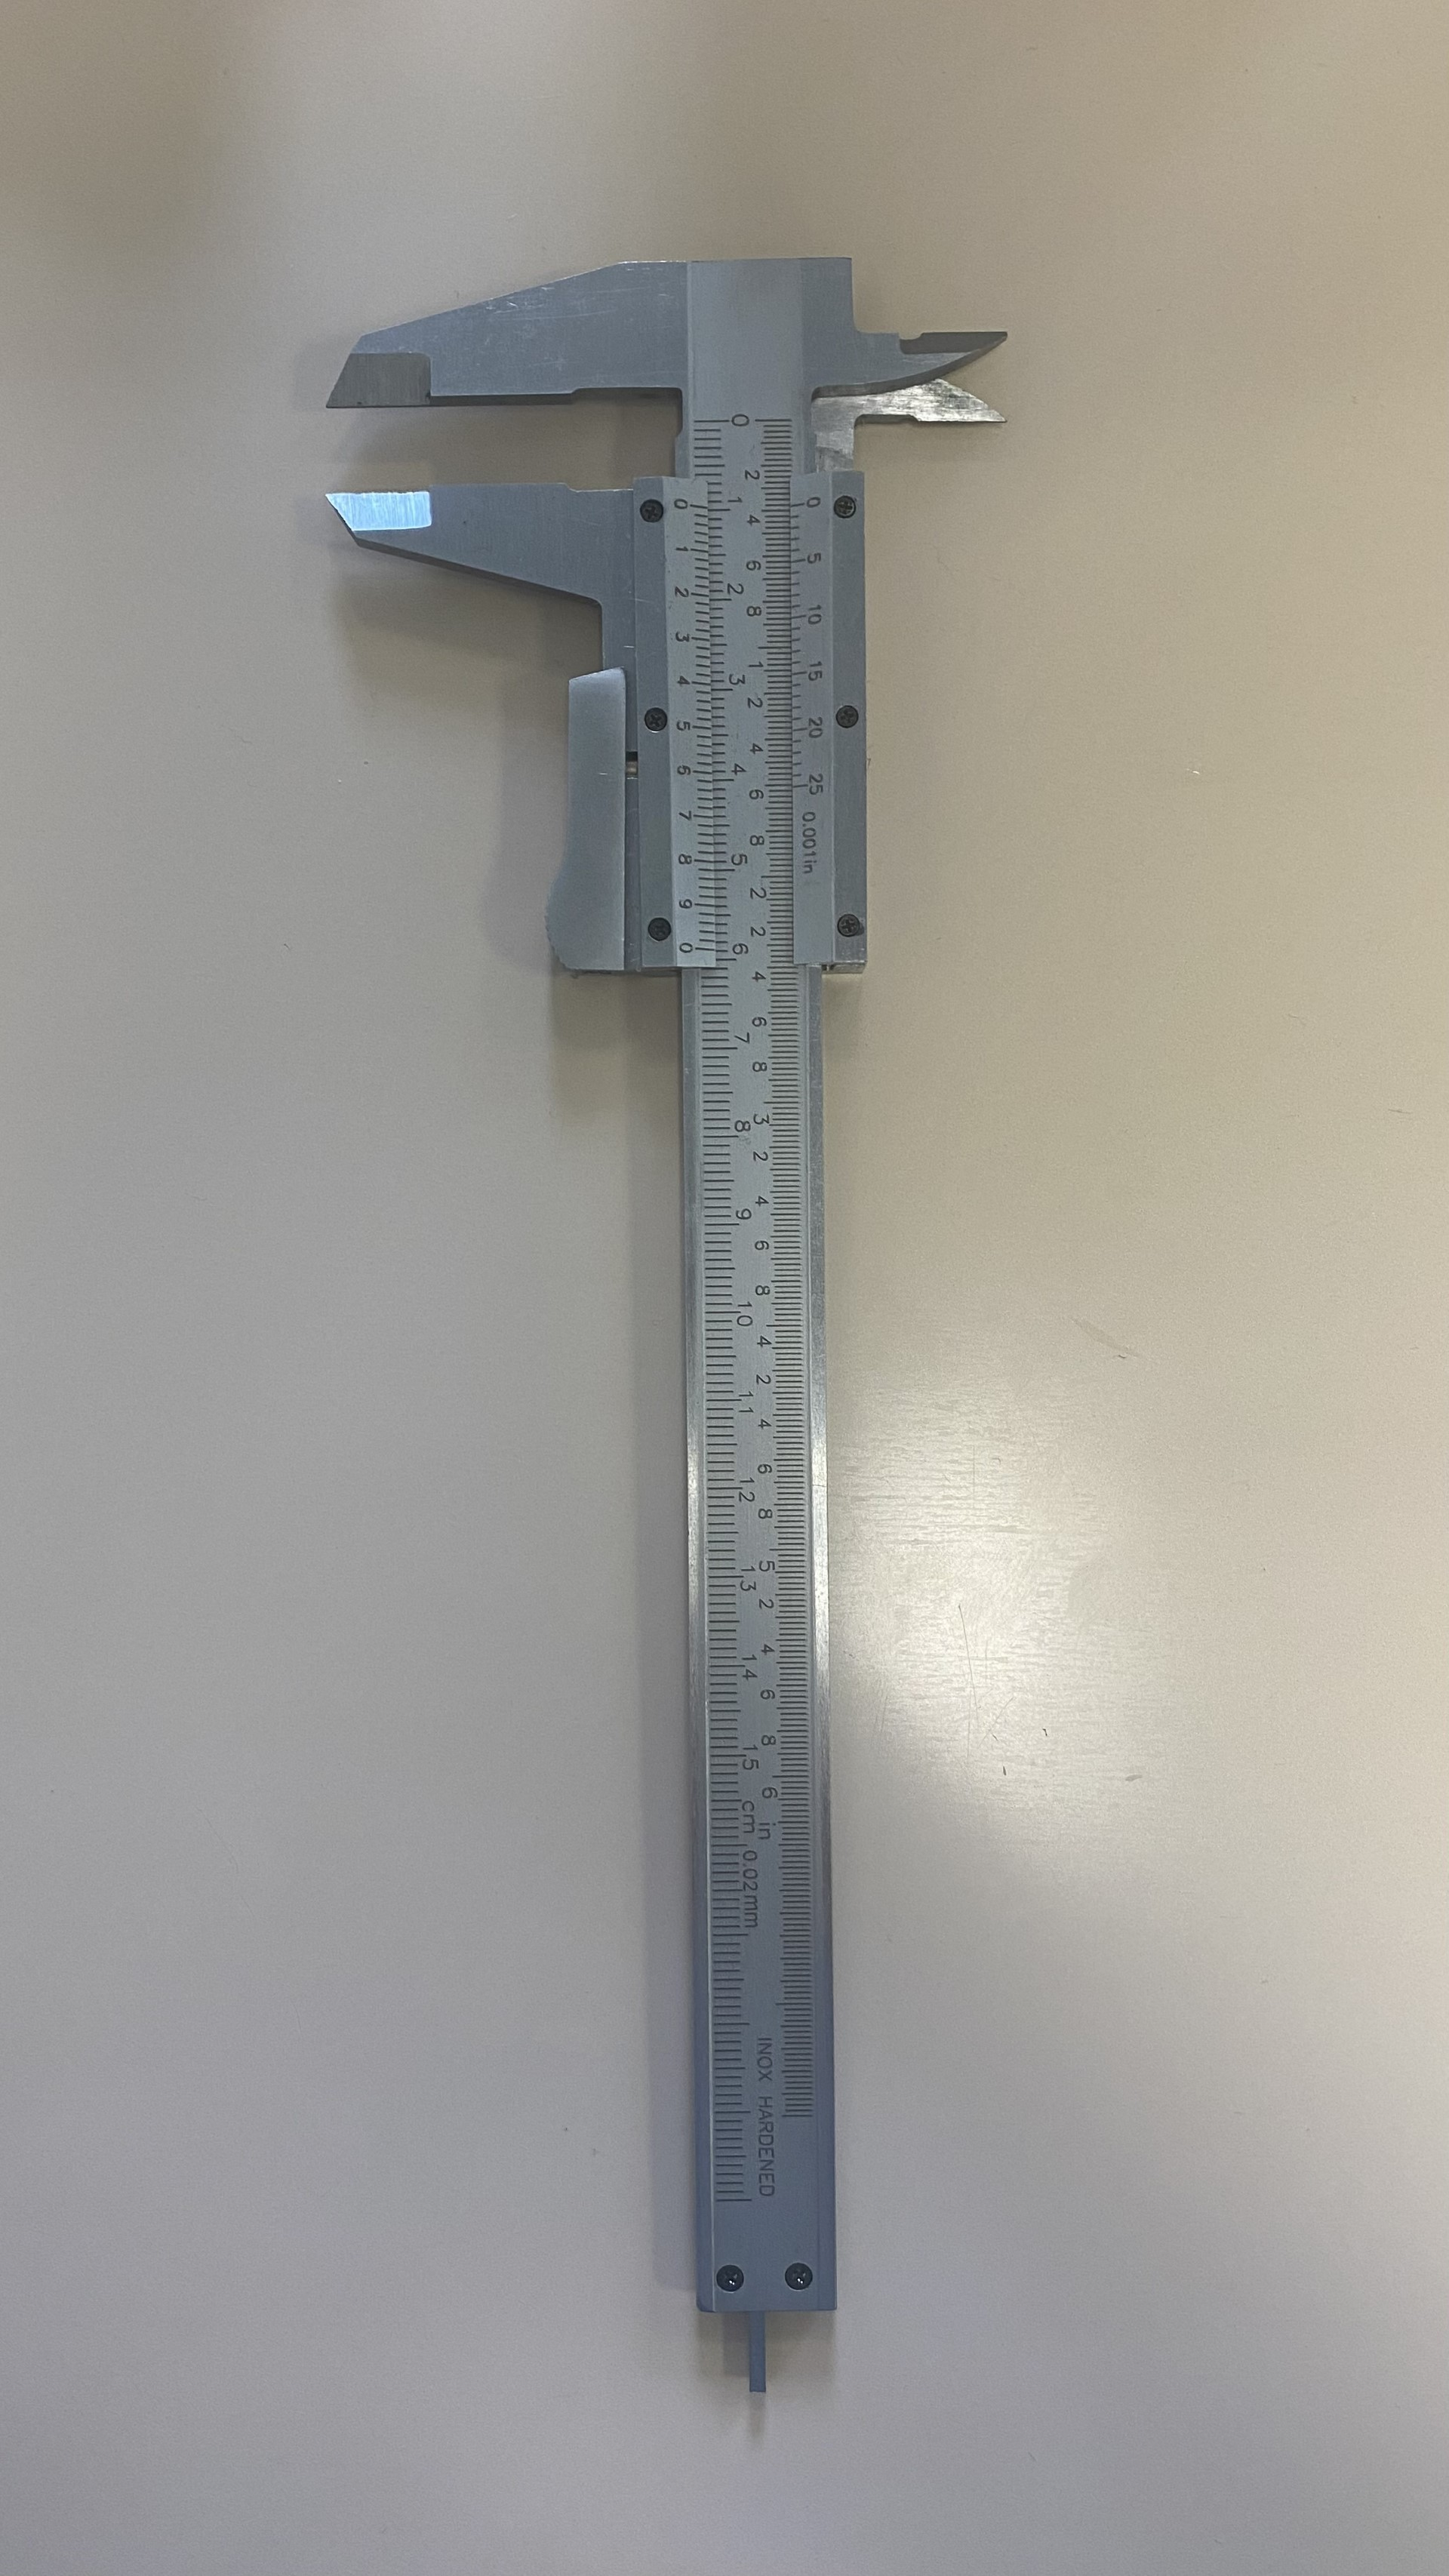
\includegraphics[width = 10cm]{calibro cinqua.jpg.jpg}
    \caption{Calibro cinquantesimale}
    \label{fig:my_label}
\end{figure}

\begin{figure}
    \centering
    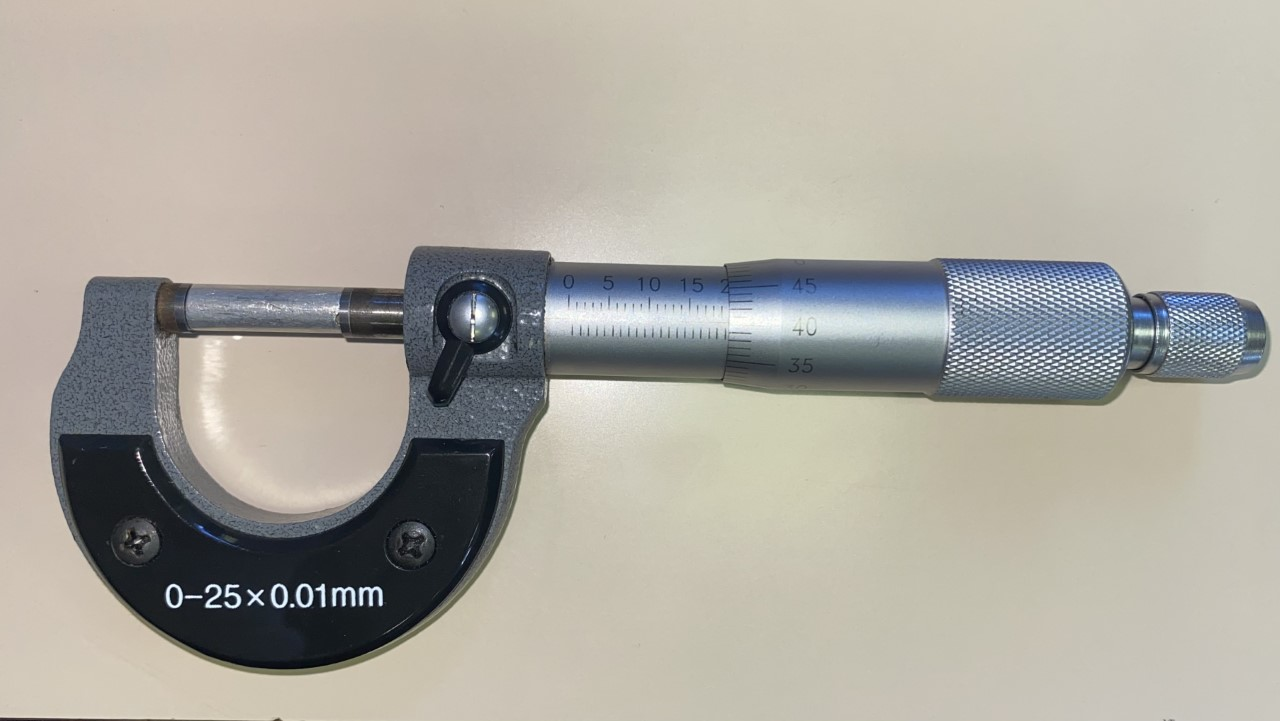
\includegraphics[width = 10cm]{palmer.jpg}
    \caption{Calibro palmer}
    \label{fig:my_label}
\end{figure}

\begin{figure} [t]
    \centering
    \includegraphics[width = 7cm]{oggetti.jpg}
    \caption{Solidi a disposizione}
    \label{fig:my_label}
\end{figure}

\FloatBarrier

\subsection{Descrizione delle misure} %4 - alessandra
Ho utilizzato il calibro cinquantesimale per le misure di altezze e basi (prisma e parallelepipedo), mentre ho usato il calibro palmer per le misure di diametro dei cilindri in quanto, avendo una superficie di contatto maggiore, ero più sicura nel prendere l'effettivo diametro del cilindro e non una sua corda. Prima di prende le misure con il palmer, mi sono assicurata che chiudendo totalmente il tamburo, lo zero della ghiera corrispondesse con l'asse graduato sul cilindro, per comprendere se ci fosse la necessità di correggere un errore di zero; tuttavia non è stato necessario poichè, appunto, lo strumento risultava ben calibrato.\\
Ho considerato come incertezza sulle misure l'incertezza dello strumento con cui ho effettuato la misura divisa per la radice di 12, poiché si tratta di strumenti digitali e quindi l'incertezza è uniforme su tutto il range di misura.\\
\vspace{1em}


\begin{tabular}{lcl}
    \toprule
    Solido & Spessore (\pm 0.006) [mm] & Altezza (\pm 0.003) [mm] & Massa (\pm 0.0003) [g]\\
    \midrule
    Cilindro 1 & 6.46 & 95.38 & 22.388\\
    Cilindro 2 & 10.82 & 37.50 & 24.605\\
    Cilindro 3 & 5.96 & 36.70 & 8.572\\
    Cilindro 4 & 10.46 & 16.00 & 10.468\\
    Prisma a base esagonale & 15.45 & 17.62 & 28.598\\
    Parallelepipedo &
    \bottomrule
\end{tabular}
(le misure delle dimensioni del parallelepipedo serviranno alla fine dell'esperimento per confrontare il valore del volume ottenuto con i dati noti e quello ottenuto a partire dalla stima della densità dell'ottone).\\
Tutte le misure sono state divise per 1000 per ottenere i valori delle lunghezze in metri e quello delle masse in Kg, così da avere la densità in $Kg/m^3$.\\

Nell'ordine, dunque, ho misurato le masse dei sei corpi di ottone, mettendo da parte quello di massa maggiore (che ho utilizzato poi per la verifica finale); di seguito ho misurato il volume e le rispettive incertezze dei volumi dei solidi, utilizzando le formule riportate nel paragrafo precedente. A questo punto, ho realizzato un fit lineare masse - volumi per stimare la densità del materiale e con quest'ultima ho misurato il volume del corpo di massa maggiore. Alla fine, ho misurato indipendentemente il volume del corpo di massa maggiore con le mie misure prese di dimensioni e massa e ho confrontato i due valori ottenuti.\\
%Di seguito, i volumi ottenuti con le rispettive incertezze:

\vspace{2em}

\subsection{Analisi dei dati - metodo di fit e grafico dei residui condotto utilizzando la funzione curve\_fit() di Python}

\label{subsec: curve-fit}
Ho utilizzato i dati raccolti per eseguire un fit tramite la funzione curve\_fit() di Python; in particolare, però, notiamo che se poniamo i volumi sulle x e le masse sulle y, gli errori sulla x non sono trascurabili per cui viene meno una delle ipotesi del fit dei minimi quadrati, cioè:
\begin{equation}
    \sigma_{y_i} >> \sigma_{x_i}(\frac{df}{dx})
\end{equation}
dove $f(x) = mx + q$ è la funzione che vogliamo fittare.\\
Per ovviare a questo problema, dunque, ho invertito le variabili, ponendo le masse sulle x e i volumi sulle y, in modo da poter trascurare gli errori sulle x.\\
Ho ottenuto i seguenti parametri di fit, dove m è proprio la stima della densità:

\begin{tabular}{l|c|l|c}
     \toprule
     Parametro di fit & valore\\
    \midrule
    $\frac{1}{\^{m}} \pm \sigma_m [m^3/Kg]$ & 1.49e-04 \pm 2e-06\\
    $\frac{1}{\^{q}} \pm \sigma_q [m^3]$ & -2.2e-07 \pm 3e-08\\
    \bottomrule
\end{tabular}
%non usare le potenze di 10 ma usare l'espressione "e-04"; errori con 1 o massimo 2 cifre significative

\begin{figure}
    \centering
    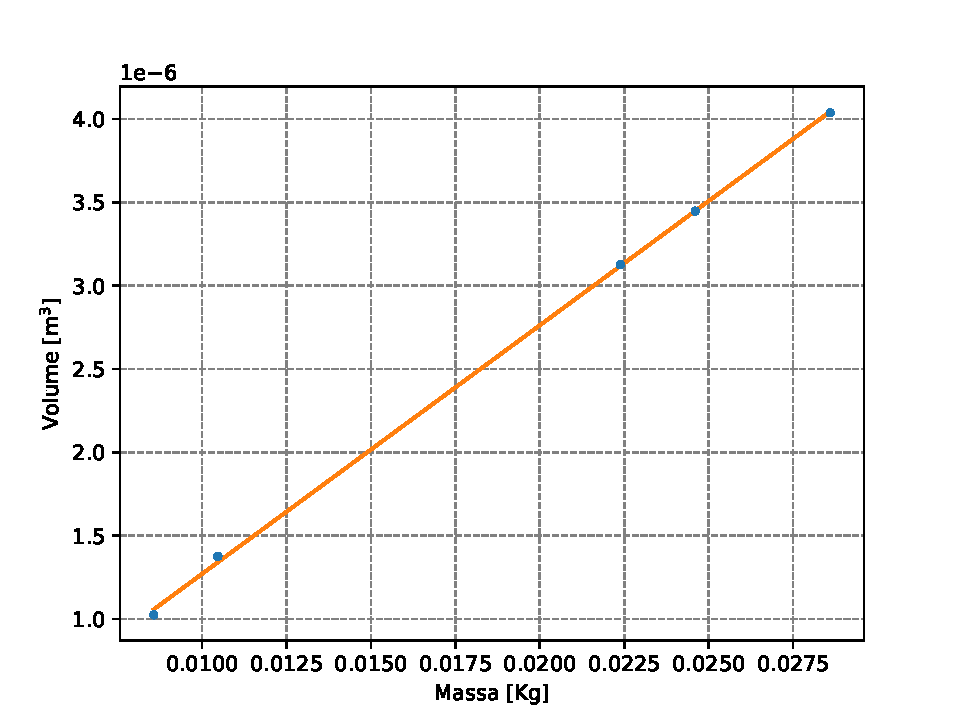
\includegraphics[width=10cm]{fit.pdf}
    \caption{Fit Massa-Volume}
    \label{fig:my_label}
\end{figure}

\begin{figure}
    \centering
    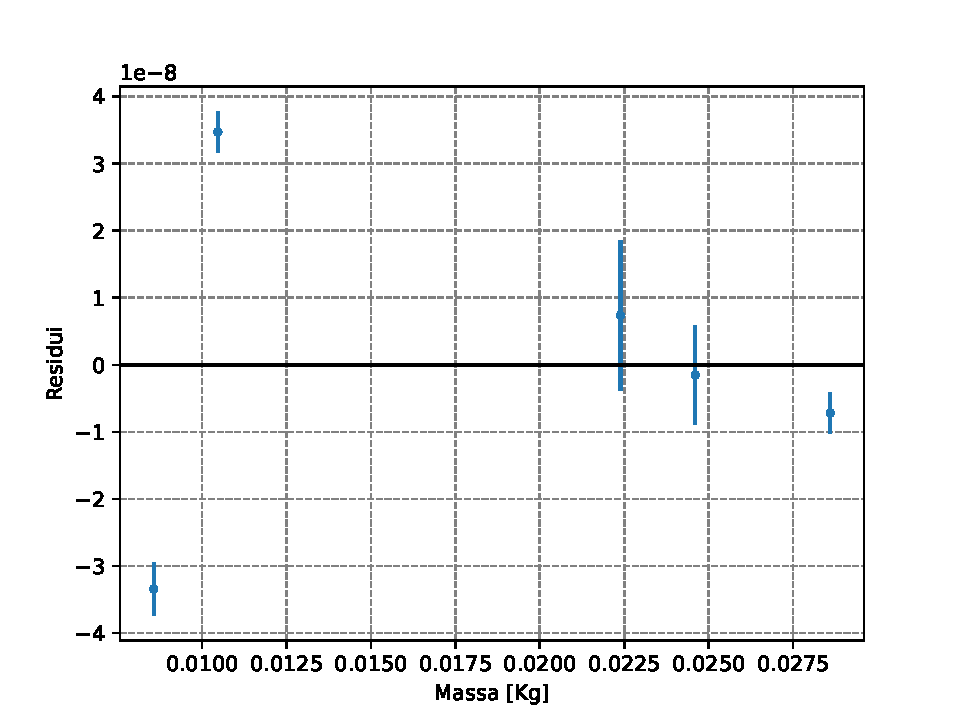
\includegraphics[width=10cm]{residui.pdf}
    \caption{Grafico dei residui}
    \label{fig:my_label}
\end{figure}

Di seguito, i dati del volume del corpo di massa maggiore ottenuti con le due misurazioni diverse:

\begin{tabular}
    \toprule
    Volume & valore [m^3]\\
    \midrule
    Volume con densità stimata & $5.21e-08 \pm 6e-08$\\
    Volume con misure dirette & $4.178e-08 \pm 2e-09$\\
\end{tabular}

\FloatBarrier

\vspace{1em}

\section{Conclusioni} 
Dunque è possibile fare una serie di commenti. Innanzitutto, trovando il valore di $\frac{1}{\hat{m}}$ è possibile confrontare il valore di densità ottenuta con quella tabulata di 8400 $Kg/m^3$.\\
Si ottiene pertanto un valore di densità di $6711 \pm 71 Kg/m^3$, che purtroppo non è compatibile con quello trovato. \\

In secondo luogo, possiamo osservare dai grafici e dai valori di \^{q} che le rette di fit hanno un'intercetta compatibile con l'origine. Per farlo, bisogna trovare $\frac{1}{\^{q}}$, poichè i valori di $\^{q}$ sono stati misurati avendo m sull'asse x e V sull'asse y (mentre l'espressione della densità è $m=\rho V$, cioè m e V sono disposti al contrario per le ragioni esposte al par. \ref{subsec: curve-fit}).\\
Inoltre, possiamo confrontare i valori di densità trovati con alcuni valori tabulati. Per le medesime ragioni sopra esposte, si calcola $\frac{1}{\^{m}}$. \\
Anche questa osservazione porta a notare che i valori ottenuti sono molto vicini a quelli tabulati, e che dunque l'esperimento effettuato rispetta il modello. Infatti,
%basta valutare la compatibilità con 0 di q stessa, non serve trovare il reciproco

\vspace{1em}

\begin{center}
\begin{tabular}{lclc}
     \toprule
     Materiale & 1/ \^{m} $[Kg/m^3]$& Valori tabulati $[Kg/m^3]$ & (1/ \^{q} \pm \sigma_q) 10^{-9} [m^3] \\
     \midrule
     Acciaio & 7818 & 7480 - 8000 & 0.038 \pm 0.29\\ 
     Alluminio & 2689 & 2710 & 0.72 \pm 0.28\\
     Ottone & 8010 & 8400 - 8700 & 0.031 \pm 0.049\\
     \bottomrule
\end{tabular}
\end{center}
%inserisci errori

\vspace{2em}

In ultima analisi, è possibile ragionare in termini delle formule \eqref{eq:1} e \eqref{eq:2} per continuare a valutare la bontà del fit realizzato per le sfere: come visto al par. \ref{subsec: curve-fit}, \\$\^{i} = 3.026 \pm 0.006$, valore che risulta molto vicino a quello atteso, cioè 3 (dove 3 è, per l'appunto, l'indice nella legge di potenza, ossia l'esponente della variabile indipendente che in questo caso è il raggio); \\
$\^{n} = 36704.62 \pm 1085.67$, valore che risulta vicino a quello dell'intercetta della retta con l'asse verticale r = 1 ($y_i = 36702.7$, che dovrebbe proprio coincidere con la norma della legge di potenza), come si vede dalla seguente immagine:

\begin{figure} [H]
    \centering
    \includegraphics[width=10cm]{Screenshot (3).png}
    \caption{Intercetta}
    \label{fig:my_label}
\end{figure}

%inserire chi quadro
%chisq = np.sum(((volumi - line(x, m, q))/errori_vol)**2)
%print(f'Chi quadro = {chisq :.1f}')
\end{document}
